\documentclass[xcolor=pdftex,dvipsnames,table,aspectratio=169]{beamer}
%\documentclass[xcolor=pdftex,dvipsnames,table,handout,aspectratio=169]{beamer}

%\setbeameroption{show notes}

\usepackage{bm,graphicx,multirow,amsmath,tikz} %fancybox,
\usepackage{color}%,textpos}
\usepackage[round]{natbib}
\usepackage[normalem]{ulem}
\usepackage{hyperref}
\usepackage{lastpage}
\usepackage{array}
\usepackage{color}
\usepackage{framed}
\usepackage{hyperref}

% Define Western colours
\definecolor{western}{rgb}{.306,.152,.524}
\definecolor{westerngray}{rgb}{.512,.508,.524}

%% Define BEAMER colours
\setbeamercolor{frametitle}{bg=western,fg=white}
\setbeamercolor{framesubtitle}{bg=western,fg=black}
\setbeamercolor{title}{fg=white,bg=western}
\setbeamercolor{author}{fg=white,bg=western}
\setbeamercolor{institute}{fg=white,bg=western}
\setbeamercolor{date}{fg=white,bg=western}

%% Set BEAMER fonts
\setbeamerfont{title}{shape=\bf}
\setbeamerfont{frametitle}{shape=\sc,size=\Large}
\setbeamerfont{framesubtitle}{shape=\sc,size=\Large}
\setbeamerfont{footline}{shape=\sc}

%% Define BEAMER toc
\setbeamercolor{section in toc}{fg=western}
\setbeamercolor{subsection in toc}{fg=westerngray}
\setbeamertemplate{sections/subsections in toc}[ball]

%% Define BEAMER background
\setbeamercolor{background canvas}{bg=white}

%% Define BEAMER footer
\setbeamertemplate{navigation symbols}{}
\setbeamercolor{footline}{fg=white,bg=western}
\setbeamertemplate{footline}{%
  \begin{beamercolorbox}[wd=\paperwidth]{footline}
    \vskip5pt

    \raisebox{.05in}{
      \scriptsize{\bf \insertshorttitle}
    }
    \hfill
    \raisebox{.05in}{
      \scriptsize{\bf \insertframenumber/\inserttotalframenumber} 
    }
    \hspace{5pt}

    \vskip5pt
  \end{beamercolorbox}
}

%% Define BLOCK environment
\setbeamercolor{block title}{fg=western}
\setbeamerfont{block title}{series=\bfseries}

%% Define ENUMERATE and ITEMIZE environements
\setbeamertemplate{itemize item}[ball]
\setbeamertemplate{enumerate item}[ball]
\setbeamercolor{item projected}{bg=western}

%% Define BEAMER toc
\setbeamercolor{sections/subsections in toc}{fg=blue!75}
\setbeamertemplate{sections/subsections in toc}[ball]

% %% Define SECTION openings
% \AtBeginSection[]{
%   \begin{frame}{\insertshorttitle}
%     \tableofcontents[currentsection,subsectionstyle=hide/hide/hide]
    
%   \end{frame}
% }

%% Define BEAMER frametitle
\addtobeamertemplate{frametitle}{
   \let\insertframetitle\insertsectionhead}{}
\addtobeamertemplate{frametitle}{
   \let\insertframesubtitle\insertsubsectionhead}{}


\makeatletter
  \CheckCommand*\beamer@checkframetitle{\@ifnextchar\bgroup\beamer@inlineframetitle{}}
  \renewcommand*\beamer@checkframetitle{\global\let\beamer@frametitle\relax\@ifnextchar\bgroup\beamer@inlineframetitle{}}
\makeatother

% Define counters for example and exercise
\newcounter{example}
\newcounter{exercise}

% Define example and exercise commands
\renewcommand{\example}
{\stepcounter{example}Example \lecturenum.\arabic{example}}
\newcommand{\examplectd}
{Example \lecturenum.\arabic{example}\ ctd}
\newcommand{\exercise}
{\stepcounter{exercise}Exercise \lecturenum.\arabic{exercise}}
\newcommand{\exercisectd}
{Exercise \lecturenum.\arabic{exercise}\ ctd}
  
\newcommand{\lecturenum}{26}

\title[SS2857]{Probability and Statistics I}
\subtitle{\lecturenum.~The $\chi^2$, $t$, and $F$ Distributions \& Distributions Based on a Normal Random Sample}

\date{Revised 02/12/24}

%% Add logo
% \titlegraphic{\includegraphics[height=2cm]{../uwo_logo_reversed}}

%% Initialize R


\begin{document}

{
\setbeamertemplate{footline}{}
\setbeamercolor{background canvas}{bg=western}

\begin{frame}
  \addtocounter{framenumber}{-1}

  \maketitle
\end{frame}
}

\begin{frame}
  \frametitle{\invisible{Hello}}
  
  \begin{center}
    \Large{\textbf{6.3 The $\chi^2$, $t$, and $F$ Distributions}}
    
    \Large{\textbf{6.4 Distributions Based on a Normal Random Sample}}

  \end{center}
  
\end{frame}

\begin{frame}
\frametitle{\invisible{Hello}}
  
  \begin{center}
    \Large{Assessing the Mean of a Distribution}
  \end{center}
\end{frame}

\section{Assessing the Mean of a Distribution}

\begin{frame}
  
  \begin{block}{\example: Do exams cause stress?}
  The normal resting heart rate of people between the ages of 18 and 25 is normally distributed with a mean of 70 beats per minute (bpm).
  
  \medskip
  
  A professor measures the heart rates of 15 of 250 students as they leave their exam. The sample mean is $\bar x=74$ bpm with a standard deviation of $s=7$ bpm. 
  
  \medskip
  
  Can the professor conclude that the mean heart rate of students leaving tests is above the normal resting heart rate? 
  
  \end{block}
\end{frame}

\begin{frame}
  \begin{block}{Distribution of the Sample Mean for a Normal Population}
    Let $X_1,\ldots,X_N$ be a random sample from a normal distribution with mean $\mu$ and variance $\sigma^2 < \infty$. 
    
    \medskip
    
    Let $\bar X_n$ be the sample mean. Then
    $$
    \frac{\bar X_n-\mu}{\sigma/\sqrt{n}} \sim \mbox{Normal}(0,1).
    $$ 
  \end{block}
\end{frame}

\begin{frame}
  \begin{block}{$t$-Distribution}
    Let $X_1,\ldots,X_N$ be a random sample from \textit{any} distribution with mean $\mu$ and variance $\sigma^2 < \infty$. 
    
    \medskip
    
    Let $\bar X_n$ be the sample mean and $S_n$ the sample standard deviation. Then
    $$
    \frac{\bar X_n-\mu}{\textcolor{red}{S_n}/\sqrt{n}} \sim t_{(n-1)}.
    $$  
  \end{block}
\end{frame}

\begin{frame}
  \begin{block}{$t$ Distribution}
    A continuous random variable, $T$, has a $t$ distribution with $\nu$ degrees of freedom if the pdf of $T$ is
    \[
      f(t)=\frac{1}{\sqrt{\pi}\nu}
      \frac{\Gamma(\frac{\nu + 1}{2})}{\Gamma(\frac{\nu}{2})}
      \left(1 + \frac{t^2}{\nu}\right)^{-(\nu + 1)/2}, \quad \textcolor{red}{-}\infty < t <\infty.
    \]
    Mathematically, we write $T \sim t_{\nu}$.
  \end{block}
\end{frame}

\begin{frame}
 \begin{block}{Properties}
        \begin{itemize}
        \item CDF: No closed form
        \item Mean: $E(T)=0$
        \item Variance: $V(T)=\frac{\nu}{\nu-2}, \quad \nu > 2$
        \end{itemize}
  \end{block}
  
  \begin{block}{Calculator}
  \begin{center}
  \url{https://stattrek.com/online-calculator/t-distribution}
  \end{center}

  \end{block}  
\end{frame}



\begin{frame}
  \begin{block}{$t$ Distribution (black) vs Standard Normal (red)}
  \begin{center}
    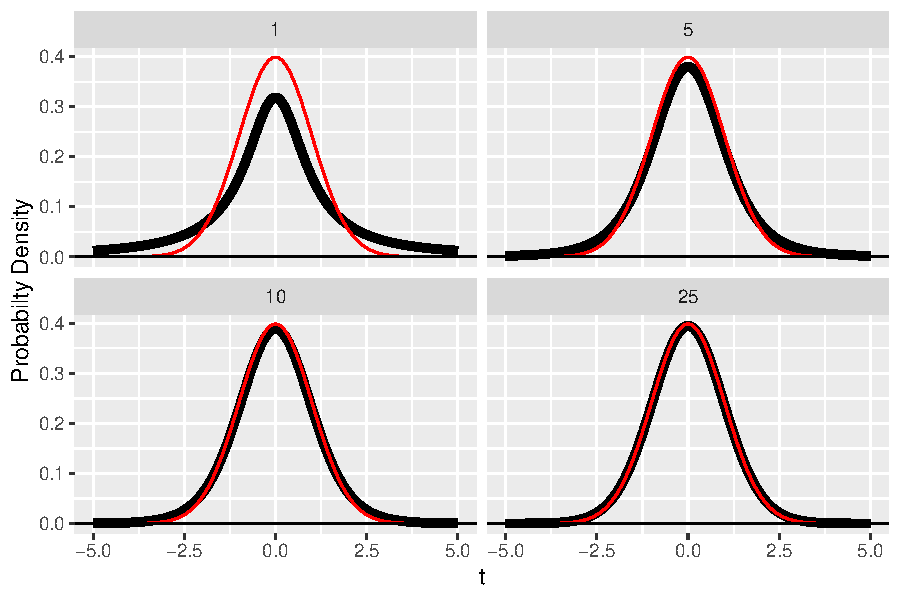
\includegraphics[height = .75\textheight]{figure/t-1}
  \end{center}
  \end{block}
\end{frame}

\begin{frame}
  
  \begin{block}{\examplectd: Do exams cause stress?}
  The normal resting heart rate of people between the ages of 18 and 25 is normally distributed with a mean of 70 beats per minute (bpm).
  
  \medskip
  
  A professor measures the heart rates of 15 of 250 students as they leave their exam. The sample mean is $\bar x=74$ bpm with a standard deviation of $s=7$ bpm. 
  
  \medskip
  
  Can the professor conclude that the mean heart rate of students leaving tests is above the normal resting heart rate? 
  
  \end{block}
\end{frame}



\begin{frame}
  \begin{block}{\examplectd: Do exams cause stress?}
  \begin{center}
    \only<1>{
    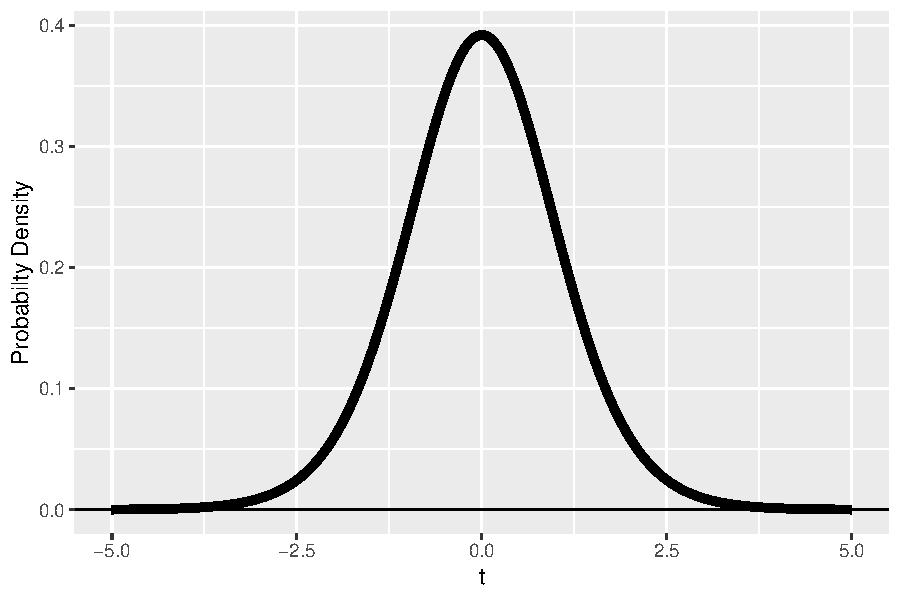
\includegraphics[height = .75\textheight]{figure/ex1-1}
    }
    \only<2>{
    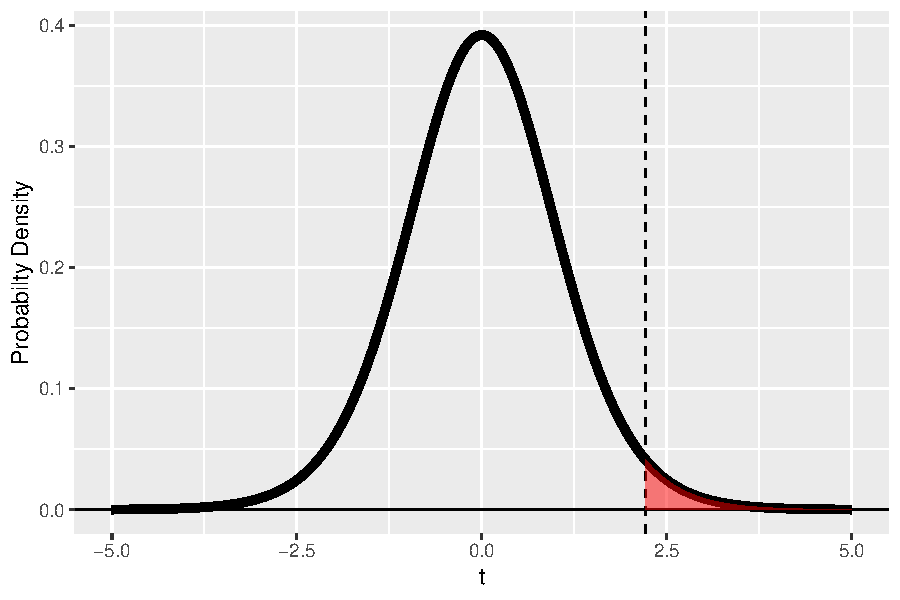
\includegraphics[height = .75\textheight]{figure/ex1-2}
    }
  \end{center}
  \end{block}
\end{frame}

\begin{frame}
\frametitle{\invisible{Hello}}
  
  \begin{center}
    \Large{Assessing the Variance of a Distribution}
  \end{center}
\end{frame}

\section{Assessing the Variance of a Distribution}

\begin{frame}

  \begin{block}{\example}
  The amount of string on a spool produced by the Acme is supposed to be normally distributed with a mean of 50~m and a standard deviation of $.1~m$. 
  
  \medskip
  
  Each day the company tests 20 randomly selected spools. Suppose they find that the observed standard deviation is .11~m.
  
  \medskip
  
  Can they conclude that the standard deviation is too high?
  \end{block}
\end{frame}

\begin{frame}

  \begin{block}{Distribution of the Sample Variance for a Normal Population}
    Let $X_1,\ldots,X_n$ be a random sample from a normal distribution with mean $\mu$ and variance $\sigma^2 < \infty$. 
    
    \medskip
    
    Let 
    $$
    S^2_n=\frac{1}{n-1}\sum_{i=1}^n(X_i -\bar X)^2
    $$
    be the sample variance. Then
    $$
    \frac{(n-1)S^2}{\sigma^2} \sim \chi^2_{n-1}
    $$ 
  \end{block}

\end{frame}

\begin{frame}
  \begin{block}{Chi-Squared Distribution (Lecture 17)}
    If $X \sim \mbox{Gamma}(\nu/2,2)$ then we say that $X$ follows a chi-squared distribution with $\nu$ degrees of freedom:
    \[
      X \sim \chi^2_\nu.
    \]
    The pdf of the chi-squared distribution is
    \[
      f(x)=\frac{1}{2^{\nu/2}\Gamma(\nu/2)}x^{(\nu/2)-1}e^{-x/2},\quad x \geq 0.
    \]
  \end{block}

\end{frame}

\begin{frame}

  \begin{block}{Properties}
%    \begin{scriptsize}
%    \begin{columns}
%      \begin{column}{.5\textwidth}
        \begin{itemize}
        \item CDF: No closed form

%        \item MGF: $M_X(t)=\frac{1}{(1-2t)^{\nu/2}}$
          
        \item Mean: $E(X)=\nu$
%        \end{itemize}
%      \end{column}
      
%      \begin{column}{.5\textwidth}
%        \begin{itemize}
        \item Variance: $V(X)=2\nu$

%        \item Skewness: $\sqrt{\frac{8}{\nu}}$

%        \item Excess Kurtosis: $\frac{12}{\nu}$
        \end{itemize}
%      \end{column}
%    \end{columns}
%  \end{scriptsize}
\end{block}

\begin{block}{Calculator}

\begin{center}
\url{https://stattrek.com/online-calculator/chi-square}
\end{center}
\end{block}
\end{frame}

\begin{frame}

  \begin{block}{\examplectd}
  The amount of string on a spool produced by the Acme is supposed to be normally distributed with a mean of 50~m and a standard deviation of $.1~m$. 
  
  \medskip
  
  Each day the company tests 20 randomly selected spools. Suppose that the observed standard deviation on one day is .11~m.
  
  \medskip
  
  Can they conclude that the standard deviation is too high?
  \end{block}
\end{frame}



\begin{frame}
  \begin{block}{\examplectd}
  \begin{center}
    \only<1>{
    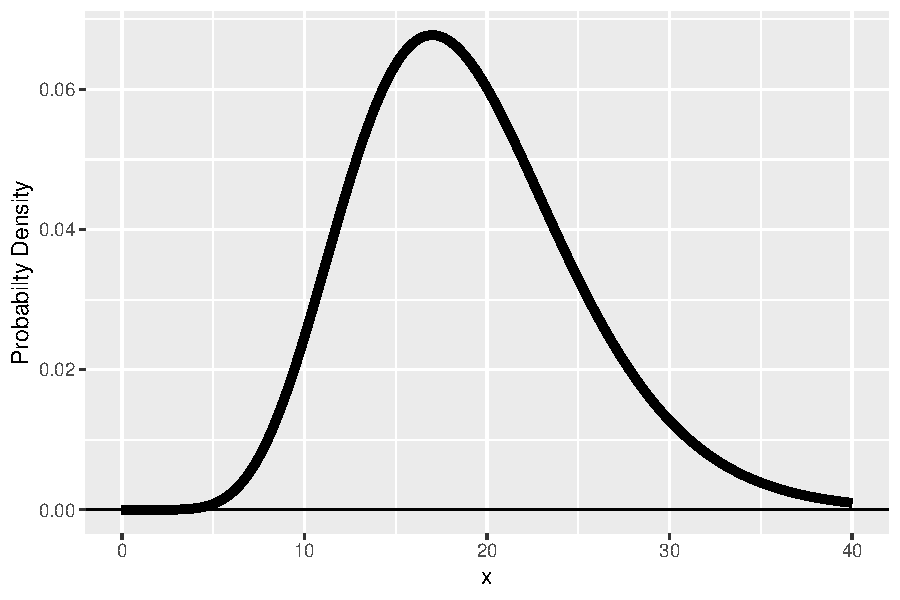
\includegraphics[height = .75\textheight]{figure/ex2-1}
    }
    \only<2>{
    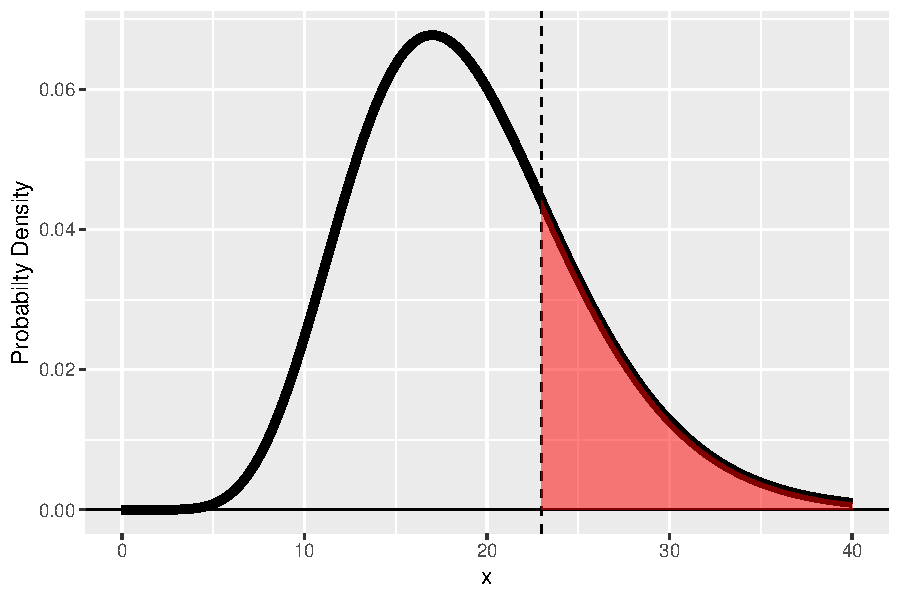
\includegraphics[height = .75\textheight]{figure/ex2-2}
    }
  \end{center}
  \end{block}
\end{frame}


\begin{frame}
\frametitle{\invisible{Hello}}
  
  \begin{center}
    \Large{Comparing the Variances of Two Distributions}
  \end{center}
\end{frame}

\begin{frame}

  \begin{block}{\example}
  The amount of string on a spool produced by the Acme is supposed to be normally distributed with a mean of 50~m. 
  
  \medskip
  
  Each day the company tests 20 randomly selected spools. Suppose that the observed standard deviation is .11~m and .09~m the next.
  
  \medskip
  
  Can they conclude that the standard deviation is higher on the first day?
  \end{block}
\end{frame}

\begin{frame}

  \begin{block}{Distribution of the Ratio of Sample Variances for two Normal Populations}
    Let $X_1,\ldots,X_n$ be a random sample from a normal distribution with mean $\mu_1$ and variance $\sigma_1^2 < \infty$ and $Y_1,\ldots,Y_m$ be a random sample from a normal distribution with mean mean $\mu_2$ and variance $\sigma_2^2 < \infty$.
    
    \medskip
    
    Let 
    $$
    S^2_1=\frac{1}{n-1}\sum_{i=1}^n(X_i -\bar X)^2
    $$
    and
    $$
     S^2_2=\frac{1}{m-1}\sum_{i=1}^m(Y_i -\bar Y)^2.
    $$
    Then
    $$
    \frac{S_1^2/\sigma_1^2}{S_2^2/\sigma_2^2} \sim F_{n-1,m-1}
    $$ 
  \end{block}

\end{frame}

\begin{frame}

  \begin{block}{Properties}
        \begin{itemize}
        \item CDF: No closed form
        \item Mean: $E(X)=\frac{\nu_2}{(\nu_2-2)}$, $\nu_2>0$
        \item Variance: $V(X)=\frac{2\nu_2^2(\nu_1+ \nu_2 + 2)}{\nu_1(\nu_2-2)^2(\nu_2-4)}$, $\nu_2>4$
        \end{itemize}
  \end{block}

    \begin{block}{Calculator}

    \begin{center}
    \url{https://stattrek.com/online-calculator/f-distribution}
    \end{center}
    \end{block}
\end{frame}

\begin{frame}

  \begin{block}{\examplectd}
  The amount of string on a spool produced by the Acme is supposed to be normally distributed with a mean of 50~m. 
  
  \medskip
  
  Each day the company tests 20 randomly selected spools. Suppose that the observed standard deviation is .11~m and .09~m the next.
  
  \medskip
  
  Can they conclude that the standard deviation is different?
  \end{block}
\end{frame}



\begin{frame}
  \begin{block}{\examplectd}
  \begin{center}
    \only<1>{
    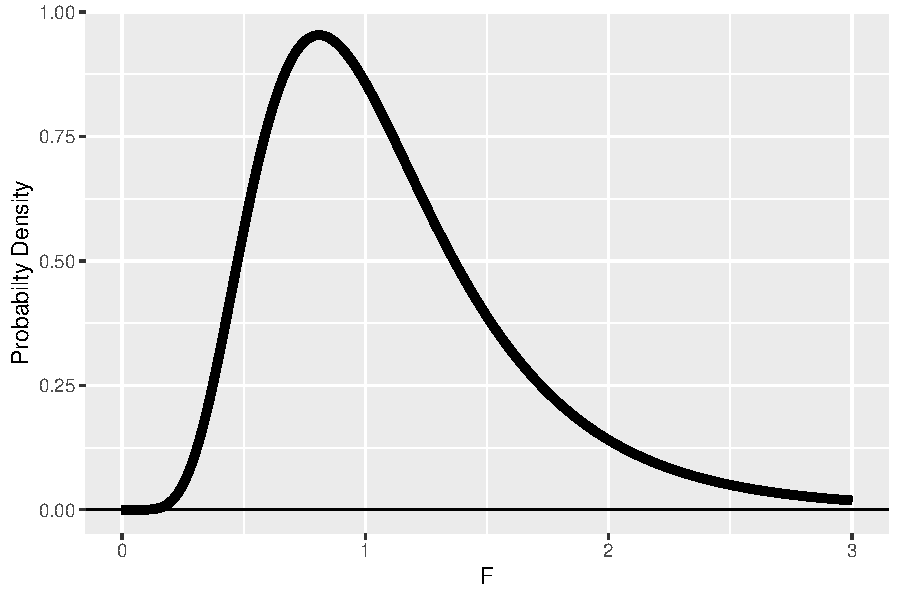
\includegraphics[height = .75\textheight]{figure/ex3-1}
    }
    \only<2>{
    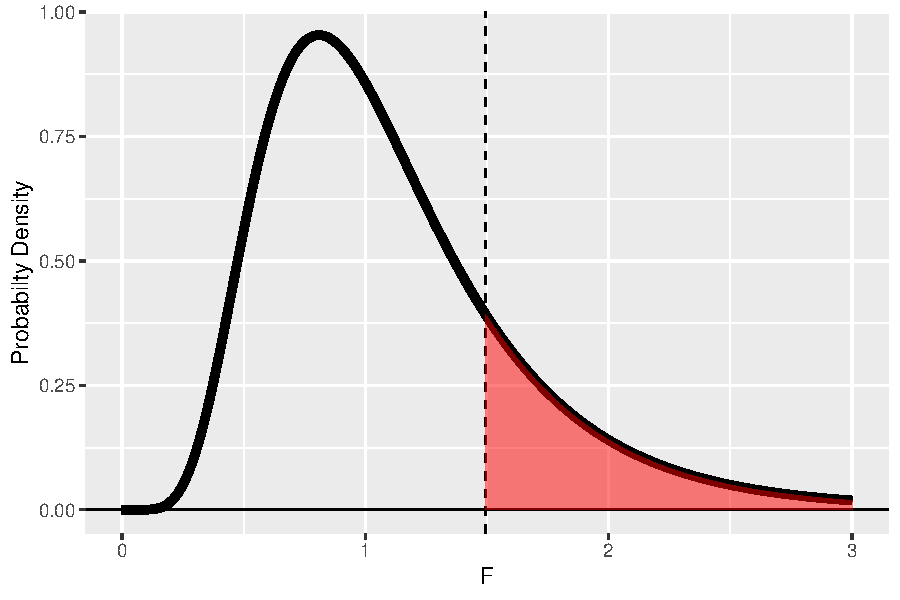
\includegraphics[height = .75\textheight]{figure/ex3-2}
    }
  \end{center}
  \end{block}
\end{frame}

\begin{frame}<handout:0>
  \begin{center}
    \Huge{\textbf{Questions?}}
  \end{center}
\end{frame}

\begin{frame}

  \begin{block}{\exercise}

  The historical average maximum daily temperature in London in October is normally distributed with a mean of 15C. Suppose that the temperatures on each of the 31 days are mutually independent\footnote{This is a highly questionable assumption.}
  \begin{enumerate}[a)]
  \item The observed mean in October of this year was 17.76C with a standard deviation of 4.59C. Is it reasonable to believe that the mean is still 15C?
  
  \item The historical standard deviation is 4C. Is it reasonable to believe that this is still true?
  
  \item The standard deviation in September of this year was 3.00C. Can we conclude that daily maximum temperatures in October are more variable than in September?
  \end{enumerate}
  \end{block}
\end{frame}

\end{document}
